\chapter{Architektura}

\section{Opis ogólny architektury systemu}

\begin{figure}[!h]
    \begin{center}
    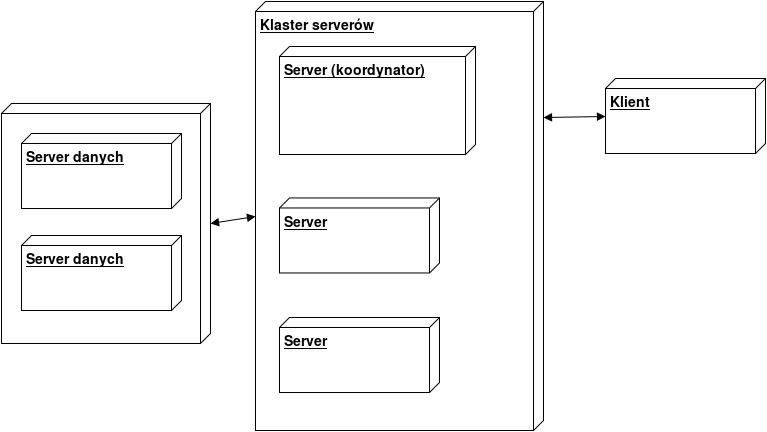
\includegraphics[angle=0,scale=0.55]{img/arch.png}
    \end{center}
    \caption{\em Schemat architektury systemu}
    \label{fig:arch}
\end{figure}


System po stronie serwerowej składa się z dwóch warstw. Wewnętrznej, która przechowuje wrażliwe informacje medyczne i zewnętrznej udostępniającej informację oprogramowaniu klienckiemu. Część wewnętrzną stanowi system rozproszonej bazy danych, a część zewnętrzną klaster serwerów.

\section{Baza danych}

\begin{figure}[!h]
    \begin{center}
    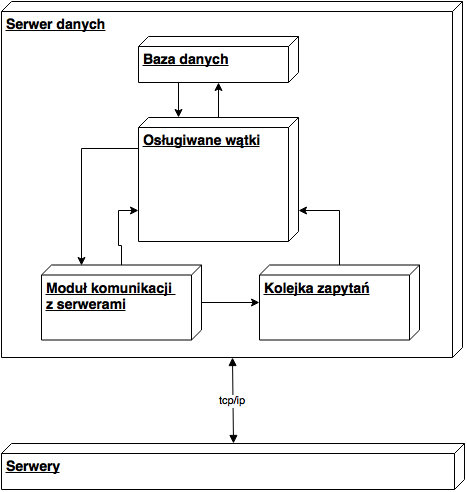
\includegraphics[angle=0,scale=0.75]{img/db.png}
    \end{center}
    \caption{\em Schemat serwera bazy danych}
    \label{fig:db}
\end{figure}

Zastosowanie prostej replikacji całego serwera danych. Poziom redundancji danych jest równy ilości serwerów danych. Zrealizowany zostanie model spójności sekwencyjnej. Każda zmiana w dowolnej bazie bazie powoduje rozpropagowanie jej na pozostałe serwery danych.
W projekcie przewidziane są dwa serwery danych, co daje redundancję równą 2.

Komunikacja z serwerami odbywa się przez tcp/ip. W komunikacji pośredniczy moduł komunikacyjny, który oczekuje na zapytania. Każde zapytanie jest obsługiwane w oddzielnym wątku. Zapytania są kolejkowanie lub odrzucane, gdy zapytań będzie za dużo. Komunikacja jest szyfrowana przy pomocy RSA.


\section{Serwer}

\begin{figure}[!h]
    \begin{center}
    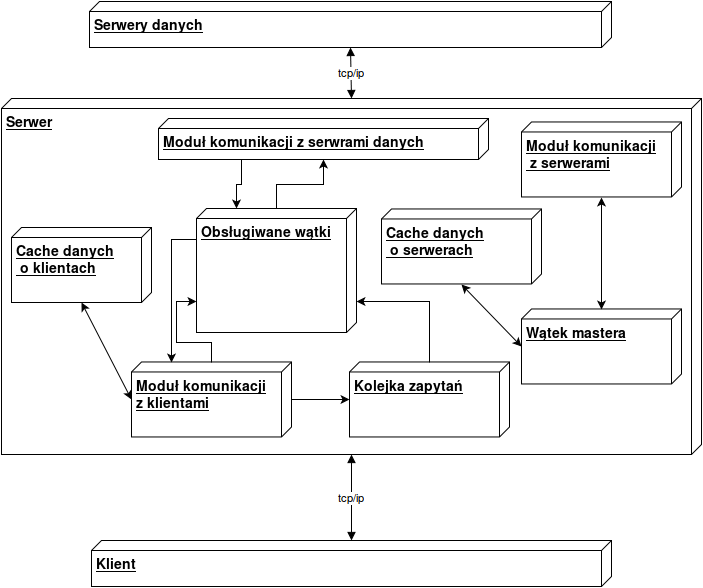
\includegraphics[angle=0,scale=0.6]{img/serv.png}
    \end{center}
    \caption{\em Schemat serwera aplikacyjnego}
    \label{fig:serv}
\end{figure}

Serwer odbiera zapytania od klienta i pobiera dane z bazy. W tym celu nasłuchuje w oczekiwaniu na połączenie od klienta. Komunikacja klient-serwer odbywa się przez tcp/ip. Po odebraniu żądania, tworzony jest nowy wątek, który realizuje zapytanie, komunikuje się z bazą danych oraz formułuje odpowiedź. Serwer może obsłuzyć ograniczoną liczbę klientów. Nadamiarowe zapytania może przekazać innym serwerom, a jeżeli wszystkie są zajęte to wstawia do kolejki oczekujących zapytań lub odsyła odpowiedni komunikat, jeżeli w kolejce nie ma miejsc.
Zadaniem serwera jest też autoryzacja łączącego się klienta, sprawdzenie jego uprawnień. Autoryzacja i uwierzytelnienie odbywa się przez podanie loginu i hasła. Gdy serwer dostanie zapytanie od niezalogowanego klienta odsyła prośbę o login i hasło. Po autoryzacji klient jest zapisywany w tablicy aktywnych klientów w cachu, następnie serwer generuje, zapisuje i wysyła token, który będzie służył do uwierzytelniania przy kolejnych żądaniach aż do momentu wylogowania lub gdy użytkownik przez określony czas będzie nieaktywny. Dane o aktywnych klientach nie są przechowywane na wszystkich węzłach, więc jeżeli jeden z nich ulegnie awarii konieczna będzie ponowna autoryzacja i uwierzytelnienie na innym węźle.
Jeden z serwerów jest koordynatorem. Koordynator kontroluje pracę pozostałych serwerów, sprawdza, czy wszystkie są dostępne, autoryzuje nowy węzeł, który chce się połączyć. Tworzy i rozsyła do wszystkich węzłów tablicę aktywności serwerów oraz serwerów danych. Sprawdzanie obecności serwerów odbywa się poprzez cykliczne odpytywanie.
Gdy master ulegnie awarii jego rolę przejmuje inny z serwerów.
Wszystkie serwery znają liczbę i adresy pozostałych. Każdy z serwerów ma przyporządkowany numer. Masterem staje się ten o najniższym numerze. Pierwszy serwer, który zauważy, że nie ma mastera wysyła komunikat do wszystkich węzłów o niższym numerze, jeżeli nikt nie odpowie to serwer staje się nowym koordynatorem i wysyła do wszystkich pozostałych węzłów informujący komunikat. Jeżeli któryś z węzłów o niższym numerze odpowie to on przejmuje kontrolę. Brak koordynatora będzie zauważony, gdy węzeł nie zostanie odpytany w odpowiednim czasie.

\subsection{Autoryzacja węzłów}
Każdy węzeł posiada nazwę oraz numer. Aby dołączyć się do klastra serwerów musi wysłać masterowi numer oraz swoją nazwę zaszyfrowaną kluczem publicznym mastera. W odpowiedzi dostaje potwierdzenie i aktualny stan systemu, aby zaktualizować listę aktywnych serwerów.  Klucze publiczne są zapisywane w plikach konfiguracyjnych serwera i klienta.

\section{Aplikacja kliencka}

\begin{figure}[!h]
    \begin{center}
    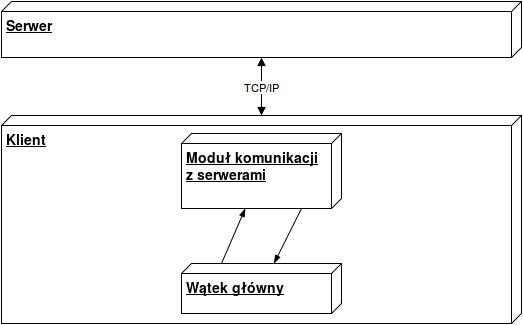
\includegraphics[angle=0,scale=0.8]{img/client.png}
    \end{center}
    \caption{\em Schemat aplikacji klienckiej}
    \label{fig:client}
\end{figure}

Zadaniem aplikacji klienckiej jest nawiązanie połączenia z jednym z serwerów. Adresy serwerów są określone w pliku konfiguracyjnym. Jeżeli połączenie z jednym z węzłów zakończy się niepowodzeniem, następuje próba połączenia się z kolejnymi. Aplikacja umożliwia zalogowanie się i dostęp do funkcji oferowanych przez API serwera. Jeżeli jakieś żądanie się nie powiedzie pomimo dostępności serwera, następuje ponowna próba, wysłania żądania ale do innego serwera.
Klient musi aktualizować listę serwerów poprzez cykliczne odpytywanie.

\section{Plik konfiguracyjny}

W pliku konfiguracyjnym klienta znajdują się adresy, porty i nazwy serwerów oraz ich klucze publiczne.
W pliku konfiguracyjnym serwerów znajdują się adresy, porty i nazwy serwerów, adresy serwerów baz danych, maksymalna liczba jednocześnie obsłużonych wątków, okres odpytywania węzłów przez serwer główny, czas trwania sesji z klientem, klucze publiczne serwerów.
